
\chapter{Material and Methods: the alignment model} \label{sec:model}
This chapter contains the material and methods necessary to understand the mathematical model used for the recovery study. The majority of the content concerns Bayesian inference, which confers a probabilistic approach to infer to learn the typical recovery curve and classify different types of recoveries. 

\section{Description} 
\subsection{Concept} 
The alignment model's objective is to draw the typical profile of a recovery. Looking at figure \ref{fig:schematics}, since patients start antibiotic treatments in different conditions, the raw patient data is unusable. However, patterns in the behaviour can be observed by aligning the antibiotic interventions to one another and averaging their values. The alignment model was used to 1) infer the profile of recovery for each type of measure, and 2) learn the recovery start date as an offset from the treatment starts for each data record.

    \begin{figure}[!h]
    \caption{Alignment model schematics}
    \centering
    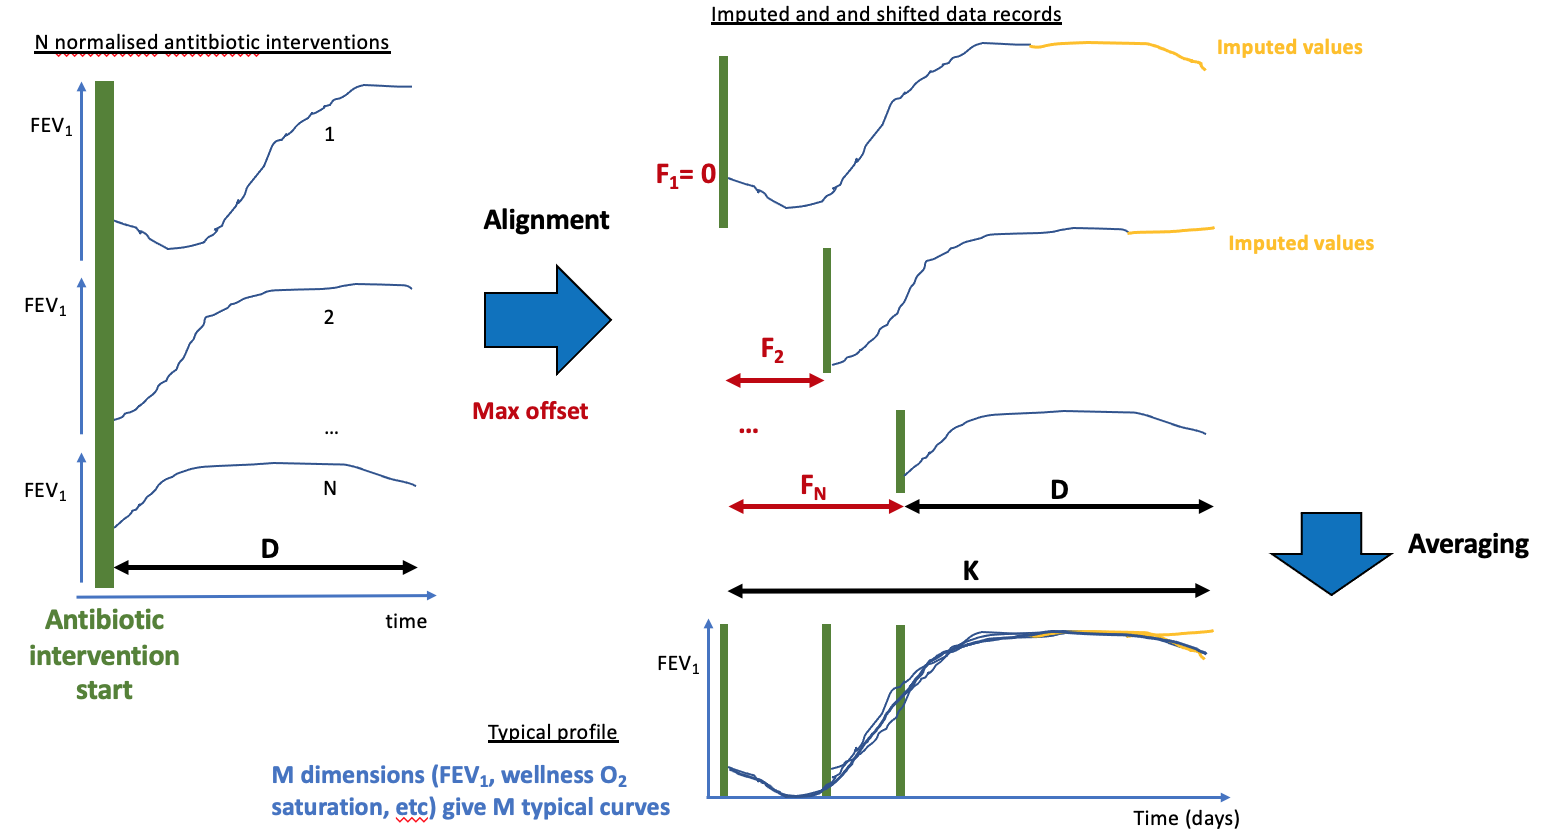
\includegraphics[width=150mm]{images/schematics.png}
    \label{fig:schematics}
    \end{figure}

\subsection{Reasons for the model}
Sutcliffe et al. \cite{damian} addressed the issue of curve alignment in their study of APEs. They proved that a probabilistic inference algorithm could learn the typical profile of an APE despite the scarcity, the noisiness, the presence of abrupt changes in the data.

The recovery analysis uses this algorithm written in MatLab. The rest of the section dives into the description and the mathematical formulation of this model. Note that it was decided to include the terminology related to the recovery to improve clarity and avoid repetitions.

\subsection{Terminology} \label{sec:datainputs}
To begin with, three main model concepts can be described:

\subsubsection{Data record}A data record, also called an (antibiotic) intervention, is a data sample of length D containing the set of home measurements performed during the period immediately following antibiotic treatment. A data record contains M times-series of the physiological data for each selected measure among the measures list introduced in table \ref{tab:measures} (FEV1, $O_2$ Saturation, Cough, Wellness, etc). The data records are $\mu$-normalised based on the patient's last stable values, this allows to easily observe full recoveries when signals come back to the stable baseline, and $\sigma$-normalised by the patient measure's mean amplitude, to harmonise data records across patients.

\subsubsection{Typical profile}The typical profile, or latent curve, of length K is the superposition of all data records, shifted by the optimal allowed offsets. The typical profile is thus longer than the data record by several days equal to the span of the offsets.

\subsubsection{Offsets}The offset values are the number of days by which a data record is allowed to be shifted upwards from the treatment start. There are exactly K-D offsets. Offset values are defined as follows. 1) for an offset of 0 the recovery starts at the same time as the announced treatment. The data record is not shifted. 2) For positive offsets the data record is shifted upwards, further away from the recovery start.

\subsubsection{Important notes:}
\begin{enumerate}
    \item The offset range is [1,K-D], but since the minimum offset is 0, for which the position of the data record is not changed, the offset values range is [0,K-D-1]. 
    \item As the data record is D-day long and the typical profile is K-day long, there are always K-D slots on the typical profile to which the data record is not contributing. Indeed, when the data record is shifted by an offset of $f$ to the right of the typical profile, the data record is solely contributing to [1+$f$;$f$+D] points on the typical profile.  
\end{enumerate}

\section{Mathematical formulation}

\subsection{Definition of the generative process} \label{sec:datagen}
The generative model creates the foundation of the inference algorithm. The machine learning model and associated variables can be represented as a factor graph (figure \ref{fig:graph}). There is one observed point – the measured value (V) - for each data record (N), for each day in the data record (D), and each type of measure (M). It was assumed that the measured value arises from the corresponding point on the typical profile for measure M, plus some Gaussian noise. Each day in a typical profile is made up of a mean value ($Z_{m,k}$), and a standard deviation from the mean ($S_{m,k}$) used to define the amount of noise added. Each typical profile can be up to K days long, K > D, where there is a pair of values of $Z_{m,k}$ and $S_{m,k}$ for each day. For each data record, there is also a latent variable for the offset ($F_n$) which is used to compare the data record to different places of the typical profile, to allow the recovery start inference. This takes the form of a probability distribution over the allowed (K-D) number of offsets.

    \begin{figure}[!h]
    \caption{Interventions by duration}
    \centering
    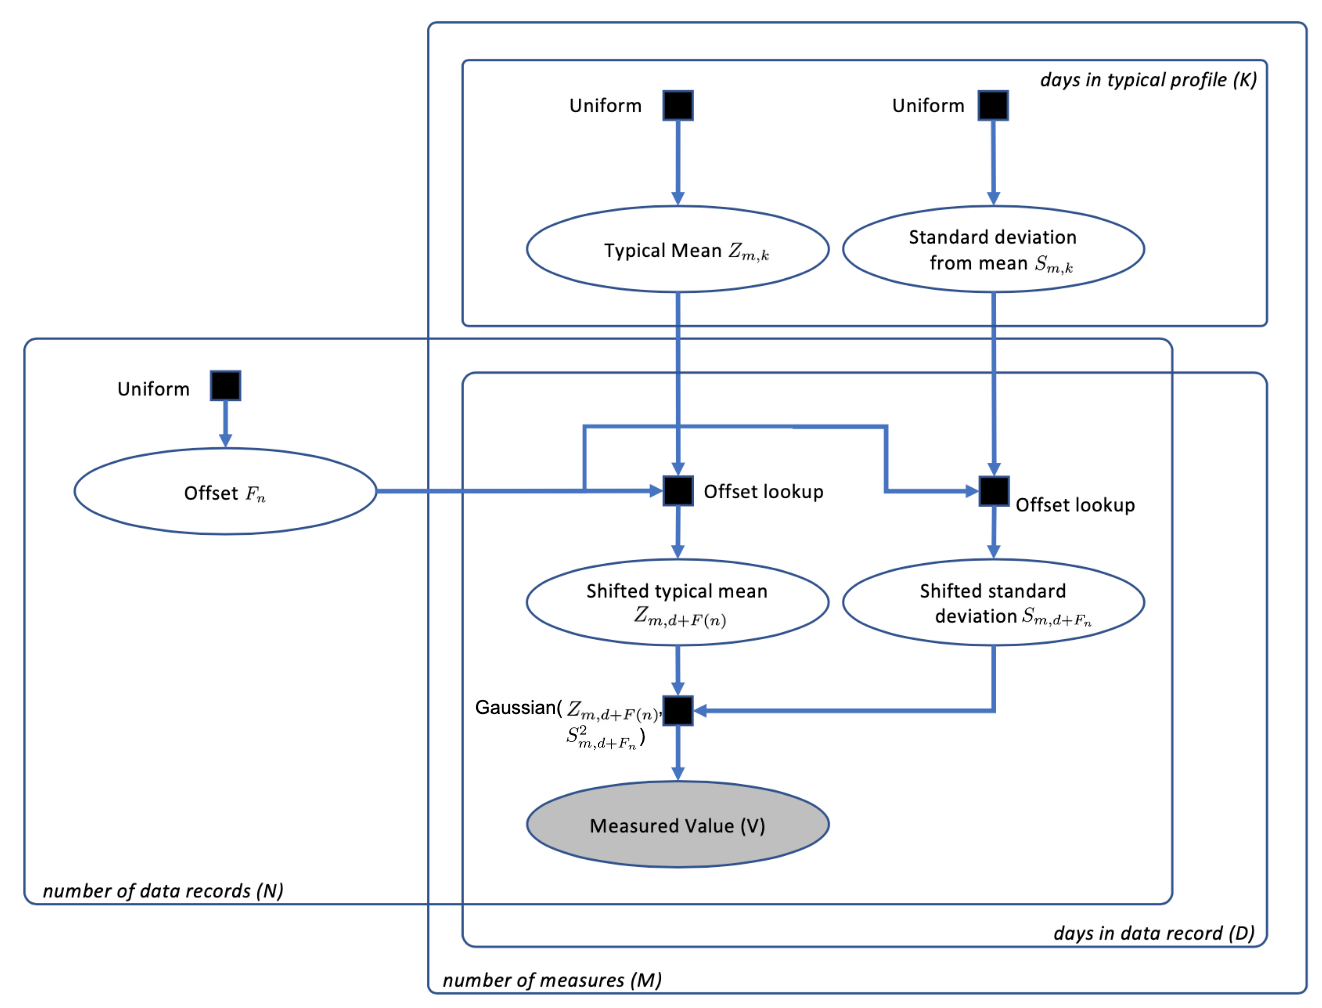
\includegraphics[width=130mm]{images/factorgraph.png}
    \label{fig:graph}
    \end{figure}
    
\begin{algorithm}[H]
\For{\mbox{each measure m = 1 to M}}{
    \For{\mbox{each day in the typical profile k:=1 to K}}{
        Draw a typical value $Z_{m,k}$ from an improper uniform distribution over $\mathbb{R}$\\
        Draw a noise standard deviation $S_{m,k}$ from an improper uniform distribution over $\mathbb{R^{+}}$
        }
    }
\For{\mbox{each data record n = 1 to N}}{
    Pick an offset $F_{n}$ from a uniform distribution $\mathcal{U}$(0,K-D-1)\\
    \For{\mbox{each day in the data record  d:=1 to D}}{
        \For{\mbox{each measure  m:=1 to M}}{
            Draw a typical value $Z_{m,k}$ from an improper uniform distribution over $\mathbb{R}$\\
            Generate a (normalised) measured value $V_{n,m,d}$ from the random variable $\mathcal{V}_{m,d+F_n}$ following a normal distribution of such that: such that $\mathcal{V}_{m,d+F_n} \sim \mathcal{N}(Z_{m,d+F(n)}, S_{m,d+F(n)}^2)$
            }
        }
    }
 \caption{Generative process}
\end{algorithm}

Note: prior to observing the data the values of $Z_{m,k}$ and $S_{m,k}$ are completely unknown. $Z_{m,k}$ could be set to any real value and $S_{m,k}$ to any real positive value. Hence, the prior probability distribution for $Z_{m,k}$ and $S_{m,k}$ have to be set to improper distributions.

\subsubsection{Sampling interpretation} 
Running this process samples from the joint distribution P($Z_{m,k}$, $F_n$, $V_{n,m,d}$). The data set is generated by repeatedly sampling values and filtering the ones that actually correspond to measured values. Eventually, this gives samples from P($Z_{m,k}$, $F_n$ | $V_{n,m,d}$).

\subsubsection{This generative process makes three assumptions:}
\begin{enumerate}
    \item For each measure, the recorded values for the period immediately following treatment are a noisy version of a single typical profile.
    \item The amount a measured value deviates from this profile is controlled by the position on the profile and is independent from one day to the next.
    \item The treatment start can happen anytime between day 1 and the maximum allowed offset (K-D).
\end{enumerate}

\subsection{Probabilistic inference algorithm}
Since the offset of each data record is unknown, the true value of the pairs ($Z_{m,k}$ and $S_{m,k}$) cannot be derived analytically. Given the available data, the objective of the inference algorithm is to reconstruct a trustworthy image of each measure's typical profile by interpolating the calculated estimates $Z_{m,k}$, $S_{m,k}$. Expectation maximisation (EM) \cite{neal_1998} \cite{billard_2018} is used to infer the data record offset probability distribution $F_n$ and compute the estimates. The EM algorithm alternately computes:
\begin{enumerate}
    \item \textbf{E-step:} The expectation of the distribution over each offset F, with Z and S fixed. This updates the probability distribution of offsets for each data record.
    \begin{equation}\label{eq:obj}
    \forall n \in [1;N], Obj_n = = -\frac{1}{2} \cdot \sum_{m=1}^M \sum_{d=1}^D \left[ A + \left( \frac{V_{n,m,d} - Z_{m,d+F_n} + B}{ S_{m,d+F_n} } \right)^2 \right],
\end{equation} 
with
\begin{equation}
    A = \ln(2\cdot \pi) + 2\cdot \ln( S_{m,d+F_n} )
\end{equation}
\begin{equation}
    B = 
    \begin{cases}
        \min (\alpha, \overline{V}_{n,m} - \overline{Z}_{m,F_n} ), & \text{for } \overline{V}_{n,m} - \overline{Z}_{m,F_n} \geq 0\\
        \max (-\alpha, \overline{V}_{n,m} - \overline{Z}_{m,F_n} ), & \text{for } \overline{V}_{n,m} - \overline{Z}_{m,F_n} < 0
    \end{cases}
\end{equation}
    \item \textbf{M-Step:} Each point in the latent profile is updated to the new maximum likelihood estimator, with the offset probability distribution fixed. This updates the typical profile.
\begin{equation}
    \forall k \in [1;K], m \in [1;M],
    \begin{cases}
        Z_{m,k}' = \frac{ \sum_{n=1}^N \sum_{f=0}^{K-D-1} V_{n,m,k-f} \cdot P(f) \cdot W(k,f) }{ \sum_{f=0}^{K-D-1} P(f)\cdot W(k,f) }\\\\
        S_{m,k}' = \frac{\left( \sum_{n=1}^N \sum_{f=0}^{K-D-1} V_{n,m,k-f} \cdot P(f) \cdot W(k,f) \right)^2}{ \sum_{f=0}^{K-D-1} P(f)\cdot W(k,f) } - Z_{m,k}^{'2}
    \end{cases}
\end{equation}
with
\begin{equation}
    W(k,f) = 
    \begin{cases}
        1, & \text{for } k > f\\
        0, & \text{for } k \leq f\\
    \end{cases}
\end{equation}
\end{enumerate}

\subsubsection{Initialisation and end-state}
The model initialisation is as follows: for each measure and data record, the probability distribution of the offsets $P(F_n)$ is uniformly distributed over the span of allowed offsets. The algorithm then starts with an M-step, and sequentially computes expectation and maximisation steps until convergence.

After convergence, the end-state of the inference algorithm is a mapping $\mathcal{F}$, defined below, that places the data record on the typical profile at the most probable offset location. A last maximisation step with $\mathcal{F}$ is performed to obtain the $Z_{m,k}$, $S_{m,k}$ of the final profile through point estimation for each offset, rather than the previously used offset probabilistic estimation. $\mathcal{F}$ has thus the $N \times K-D$ possibilities.
\begin{equation}
    \mathcal{F} : [1;N] \longrightarrow [0;K-D-1],  n \longmapsto F_n, F_n = \argmax_{[1;K-D]}(P(F_n)))-1
\end{equation}
\textit{The objective of the algorithm is to find $\mathcal{F}$ that minimises the squared sum of distances between each shifted data record and the typical profile.}

\subsubsection{Derivation of the E-step}
For each data record n, given the set of measured values $V_n$, and the set of parameters Z and S fixed from the previous M-step, one can compute the posterior distribution according to Bayes theorem \cite{olhede_2018}:

\begin{equation}
    P(F_n|V_n,Z,S) = \frac{P(V_n|F_n,Z,S) \cdot P(F_n)}{P(V_n,Z,S)}
\end{equation}
Since the prior distribution for the offsets is uniform, and $P(V_n,Z,S)$ is fixed,
\begin{equation}
    P(F_n|V_n,Z,S) \propto P(V_n|F_n,Z,S)
\end{equation}
The total probability of observing the set $V_n$ given $F_n$, Z, and S fixed is the likelihood function. As it was assumed that the measured values from the set $V_n$ are identically and independently distributed, the likelihood function is the product of the  probability distributions of the random variables $\mathcal{V}_n$ from which they are drawn. Hence the probability distribution for the offsets writes:
\begin{equation}
    P(F_n|V_n,Z,S) = \prod_{m=1}^M \prod_{d=1}^D P(V_{n,m,d}|F_n,Z_{m,d+F_n},S_{m,d+F_n})
\end{equation}
\begin{equation}
    P(F_n|V_n,Z,S) = \prod_{m=1}^M \prod_{d=1}^D \frac{1}{ \sqrt{2\cdot\pi\cdot S_{m,d+F_n}^2} } \cdot exp \left[ -\frac{1}{2} \cdot \left(\frac{V_{n,m,d} - Z_{m,d+F_n}}{ S_{m,d+F_n} }\right)^2 \right]
\end{equation}
In the log space, the objective function $Obj_n$ is obtained by computing the error between the shifted data record measures' time-series and the typical profile:
\begin{equation}
    \forall n \in [1;N], Obj_n = \ln(P(F_n|V_n,Z,S)) = -\frac{1}{2} \cdot \sum_{m=1}^M \sum_{d=1}^D \left[ A + \left( \frac{V_{n,m,d} - Z_{m,d+F_n}}{ S_{m,d+F_n} } \right)^2 \right],
\end{equation} 
with $ A = \ln(2\cdot \pi) + 2\cdot \ln( S_{m,d+F_n} )$

\subsubsection{Derivation of the M-step}
Given the offsets probability distribution $P(F_n)$, Z and S are updated to Z' and S' via maximum likelihood optimization. 
\begin{equation}
    \begin{cases}
        Z' = \argmax_Z(P(F_n|Z,V_n)) \\
        S' = \argmax_S(P(F_n|S,V_n))\\
        % note how to calculate the likelihood function?
    \end{cases}
\end{equation}

It corresponds to a variation of the maximum likelihood estimator for the normal distribution calculated for each offset and weighted by the probability distribution of the current offset:
\begin{equation}
    \forall k \in [1;K], m \in [1;M],
    \begin{cases}
        Z_{m,k}' = \frac{ \sum_{n=1}^N \sum_{f=0}^{K-D-1} V_{n,m,k-f} \cdot P(f) \cdot W(k,f) }{ \sum_{f=0}^{K-D-1} P(f)\cdot W(k,f) }\\\\
        S_{m,k}' = \frac{\left( \sum_{n=1}^N \sum_{f=0}^{K-D-1} V_{n,m,k-f} \cdot P(f) \cdot W(k,f) \right)^2}{ \sum_{f=0}^{K-D-1} P(f)\cdot W(k,f) } - Z_{m,k}^{'2}
    \end{cases}
\end{equation}
where W(k,$f$) is used to avoid pulling measures prior to treatment start into the typical profile, which were recorded during an APE. The measured values on the right side are pulled since they are still part of the recovery as explained in \ref{sec:numstability}.
\begin{equation}
    W(k,f) = 
    \begin{cases}
        1, & \text{for } k > f\\
        0, & \text{for } k \leq f\\
    \end{cases}
\end{equation}

\subsection{Model extensions}
The model was extended to improve its performance and to enable multiple classes inference.

\subsubsection{Vertical shift} \label{sec:vshift}
The quality of the model highly relies on the $\mu$-normalisation of the data records. To describe this, the objective function can be rewritten by decomposing the data record and typical profile values with their mean and rest. For the data record n and measure m, $ \overline{V}_{n,m} = 1/D \cdot \sum_{d=1}^D V_{n,m,d} $ the measured value becomes $ V_{n,m,d} = \overline{V}_{n,m} + \widetilde{V}_{n,m,d}$. Similarly for the mean of the indexed typical profile values, one obtains:
\begin{equation}
    \forall n \in [1;N], Obj_n \propto \sum_{m=1}^M \sum_{d=1}^D \left[ A + \left( \frac{\overline{V}_{n,m} - \overline{Z}_{m,F_n} + \widetilde{V}_{n,m,d} - \widetilde{Z}_{m,d+F_n}}{ S_{m,d+F_n} } \right)^2 \right]
\end{equation}

If $ \exists N_1 \subset [1;N],  \forall n \in N_1 \overline{V}_{n,m} - \overline{Z}_{m,F_n} >> \widetilde{V}_{n,m,d} - \widetilde{Z}_{m,d+F_n},$ then $ \forall n \in N_1 V_{n,m,d} - Z_{m,d+F_n} \approx \overline{V}_{n,m} - \overline{Z}_{m,F_n}  $. An incorrect vertical alignment of a data record during the $\mu$-normalisation would lead the objective function to overly focus on the remaining vertical shift $\overline{V}_{n,m} - \overline{Z}_{m,F_n}$, instead of the difference in behaviour over time characterised by $\widetilde{V}_{n,m,d} - \widetilde{Z}_{m,d+F_n}$. Taken to the extreme, the objective function will be close to constant for each tested offset $F_n$ thus bringing its probability distribution close to uniform. The related data record will have a shallow contribution during the maximisation step, and its matching offset is likely to be poorly chosen. In this case, reducing or cancelling the difference of means $\overline{V}_{n,m} - \overline{Z}_{m,F_n}$ can strengthens the contrast in P($F_n$) which allows for a better decision making for the best matching offset. This action is defined as "vertical shift".

The suggested solution is to implement a correction term B to reduce or cancel the remaining vertical shift after $\mu$-normalisation, up to a maximum realistic value $\alpha$ that has to be optimised during the utilisation of the model. The updated objective function becomes:

\begin{equation}
    \forall n \in [1;N], Obj_c,n = -\frac{1}{2} \cdot \sum_{m=1}^M \sum_{d=1}^D \left[ A + \left( \frac{V_{n,m,d} - Z_{m,d+F_n} + B }{ S_{m,d+F_n} } \right)^2 \right],
\end{equation} 
where:
\begin{equation}
    B = 
    \begin{cases}
        \min (\alpha, \overline{V}_{n,m} - \overline{Z}_{m,F_n} ), & \text{for } \overline{V}_{n,m} - \overline{Z}_{m,F_n} \geq 0\\
        \max (-\alpha, \overline{V}_{n,m} - \overline{Z}_{m,F_n} ), & \text{for } \overline{V}_{n,m} - \overline{Z}_{m,F_n} < 0
    \end{cases}
\end{equation}

\subsubsection{Smoothing}
Due to the relative scarcity of data, normal day-to-day fluctuations in the measurements were causing the typical profile to become noisy, leading to poor convergence. To overcome this problem, a 5-day mean window smoothing was applied to the typical profiles only when calculating the offset distributions in the E-step. Note that the resulting typical profiles produced by the model have not had smoothing applied.

\subsubsection{Handling numerical stability} \label{sec:numstability}
The scarcity of data also meant that one had to be careful to avoid numerical stability issues when calculating Z and S from few data values. This occurred primarily for the left-most and right-most points of the inferred typical profiles, which have the fewest underlying data records contributing to them. 

For the right-most points, stability issues were avoided by making use of additional data points to the right of (i.e. later than) the data record since these data points were readily available in the study data set. This is already implemented in the M-step with the function W(k,$f$).

The left-most points could not be handled in the same way, because the data to the left of (i.e. earlier than) the data record is before treatment has started. The patient is thus in an exacerbation period. So, as an alternative solution, if the number contributing fell below 5, then adjacent points on the data record were borrowed to maintain a sufficient number of underlying data points. This procedure maintained numerical stability while causing very minor changes to the inferred profiles.

%\subsubsection{Outliers handling}
%TODO

\subsubsection{Multiple classes} \label{sec:multiclass}
The algorithm was extended to be able to infer (C) different profiles. During the expectation step, data records are assigned to the best matching latent curve (c), which is the curve with the minimum objective function. An additional variable $\psi \in [1; C]^N$ is introduced. It stores the class assignment of each data record as defined in \ref{eq:psi}. The vectors Obj, Z, S are extended to another dimension to allow the choice of the latent curve.\\\\
\textit{Updated E-step}: \\
1) Compute the objective function for all classes and interventions.
\begin{equation}\label{eq:multiobj}
    \forall c \in [1;C], \forall n \in [1;N], Obj_{c,n} = -\frac{1}{2} \cdot \sum_{m=1}^M \sum_{d=1}^D \left[ A + \left( \frac{V_{n,m,d} - Z_{c,m,d+F_{c,n}} + B }{ S_{c,m,d+F_{c,n}} } \right)^2 \right],
\end{equation} 
where: $ A = \ln(2\cdot \pi) + 2\cdot \ln( S_{m,d+F_{c,n}} )$,
\begin{equation}
    B = 
    \begin{cases}
        \min (\alpha, \overline{V}_{n,m} - \overline{Z}_{m,F_{c,n}} ), & \text{for } \overline{V}_{n,m} - \overline{Z}_{m,F_{c,n}} \geq 0\\
        \max (-\alpha, \overline{V}_{n,m} - \overline{Z}_{m,F_{c,n}} ), & \text{for } \overline{V}_{n,m} - \overline{Z}_{m,F_{c,n}} < 0
    \end{cases}
\end{equation}
2) Assign the data record n to the best matching curve:
\begin{equation} \label{eq:psi}
    \forall n \in [1;N], \psi_n = \argmin_{[1;C]}Obj_{c,n}
\end{equation} \\\\
\textit{Updated M-step}:
\begin{equation}
    \forall k \in [1;K], m \in [1;M],
    \begin{cases}
        Z_{c,m,k}' = \Psi(c)\cdot \frac{ \sum_{n=1}^N \sum_{f=0}^{K-D-1} V_{n,m,k-f} \cdot P(f) \cdot W(k,f) }{ \sum_{f=0}^{K-D-1} P(f)\cdot W(k,f) }\\\\
        S_{c,m,k}' = \Psi(c)\cdot \frac{\left( \sum_{n=1}^N \sum_{f=0}^{K-D-1} V_{n,m,k-f} \cdot P(f) \cdot W(k,f) \right)^2}{ \sum_{f=0}^{K-D-1} P(f)\cdot W(k,f) } - Z_{c,m,k}^{'2}
    \end{cases}
\end{equation}
where
\begin{equation}
    \Psi(c) = 
    \begin{cases}
        1, & \text{for } \psi_n = c \\
        0, & \text{for } \psi_n \neq c\\
    \end{cases}
\end{equation}
\begin{equation}
    W(k,f) = 
    \begin{cases}
        1, & \text{for } k > f\\
        0, & \text{for } k \leq f\\
    \end{cases}
\end{equation}\\\\
\textit{The end-state becomes a combination of two mappings: $\mathcal{C}$ assigns each data record to a class number and $\mathcal{F}$ provides the best offset for each data record:}
\begin{equation}
    \mathcal{C} : [1;N] \longrightarrow [1;C],  n \longmapsto \psi_n, \psi_n = \argmin_{[1;C]}Obj_{c,n}
\end{equation}
\begin{equation}
    \mathcal{F} : [1;N] \longrightarrow [0;K-D-1],  n \longmapsto F_{\psi_n,n}, F_{\psi_n,n} = \argmax_{[1;K-D]}(P(F_{\psi_n,n})))-1
\end{equation}
%\subsection{Peusocode}
%TODO

\newpage